\documentclass[14pt]{article}
\usepackage{hyperref}
\usepackage[utf8x]{inputenc}
\usepackage[english,russian]{babel}
\usepackage{cmap}
\usepackage{amsmath}
\usepackage{graphicx}
\usepackage{amssymb}
\graphicspath{ {./q1_img/} }
\usepackage[left=2cm,right=2cm,
    top=2cm,bottom=2cm,bindingoffset=0cm]{geometry}

\title{Билеты по математическому анализу для коллоквиума 14 ноября. Часть I }
\author{Шишминцев Дмитрий Владимирович}

\begin{document}
    \maketitle
    \tableofcontents
    \newpage
    
    \section{Множества и операции над ними}
        \textsc{(Условно) Множество  }
         - совокупность некоторых объектов определенных по одному признаку. \\
        $ a \in A $ - элемент a принадлежит множеству A \\ 
        $ a \notin A $ - элемент a не принадлежит множеству A \\ 
        $ A \subset B $ - множество A является подмножеством B \\
        \\
        \textsc{Равенство множеств: } Множества равны если каждый элемент множества A является элементом множества B и наоборот \\
        $A = B \Leftrightarrow \begin{cases}
            x \in A \Rightarrow x \in B \\ 
            x \in B \Rightarrow x \in A
        \end{cases}$\\
        \\
        \textsc{Операции над множествами:}
        \begin{itemize}
            \item Пересечение множеств: $ A \cap B = \{ x| x \in A$ и $x \in B \}$ - коммутативно и ассоциативно
            \item Объединение множеств: $ A \cup B = \{ x | x \in A$ или $x \in B \}$ - коммутативно и ассоциативно
            \item Разность множеств: $ A \backslash B = \{ x | x \in A $и$ x \notin B \} $
            \item Симметричная разность: $ A \bigtriangleup B = (A \backslash B) \cap (B \backslash A)$
            \item Декартово произведение множеств: $ A \times B = \{(a; b) | a \in A, b \in B \}$
        \end{itemize}
           
    \section{Отображения и функции}
        \textsc{Отображение (функция) } - правило по которому $ \forall x \in A \exists ! y \in B $ \\
        \\
        Варианты функциональных отображений $F : X \rightarrow Y $
        \begin{itemize}
            \item Функция F сюръективна, если $ \forall y \in Y \exists x \in X :y = F(x)$ - каждый элемент множества Y является прообразом хотя бы одного элемента множества X
            \item Функция F инъективна, если $ \forall x \in X \exists y \in Y : y = F(x) $ - разные элементы множества X переводятся в разные элементы множества Y
            \item Функция F биективна, если она сюръективна и инъективна одновременна
        \end{itemize}
        \begin{center}
            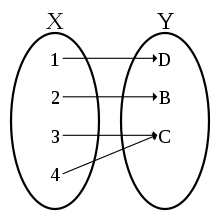
\includegraphics[scale=0.27]{2-1} 
            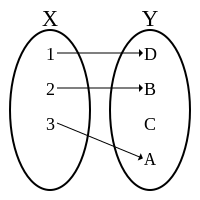
\includegraphics[scale=0.3]{2-2}
            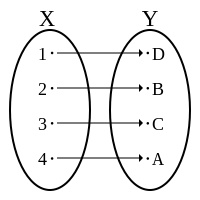
\includegraphics[scale=0.3]{2-3}    
        \end{center}
        
    \section{Эквивалентность, счетность, мощность континума}    
        \textsc{Мощность множества: } $|A|$ - число элементов входящих в множество A \\   
        \textsc{Эквивалентность множеств:} множества эквивалентны $(A \sim B)$ если $|A| = |B|$ \\
        \textsc{Счетность множество: } бесконечное множество, элементы которого можно пронумеровать натуральными числами \\
        \textsc{Мощность континуума: } мощность множества всех вещественных чисел 
 
    \section{Теорема Кантора-Бернштейна и сравнение мощности множеств}  
        \textsc{Теорема Кантора-Бернштейна} 
        \begin{enumerate}
            \item Если $A \sim B'$ (где $B' \subset B$) и $B \sim A'$ ( где $A' \subset A $) $\rightarrow A \sim B$    
            \item Если $A \subset B \subset C$, причем $A \sim C$, то $A \sim B$
        \end{enumerate}
        \textsc{Сравнение мощностей множеств:} Если множества $A$ и $B$ неэквивалентны, но $\exists B' \subset B: B' \sim A $ и $\nexists  A' \subset A: A' \sim B$, то будем считать, что $|A|<|B|$

    \section{Множество вещественных чисел и его аксиоматика}
        \textsc{Вещественные числа $\mathbb{R}$:} бесконечные десятичные дроби вида $\pm a_0,a_1a_2a_3....$, где выбран определенный знак: + или -, $a_0 \in \mathbb{N} \cup \{0\}$, а все десятичные символы $a_1, a_2...$ - цифры от 0 до 9, т.е. $\forall n \in \mathbb{N} \rightarrow a_n \in \{0,1,2,...,9\}$
        \textsc{Аксиоматика: }
            \begin{enumerate}
                \item Линейность: если $x \neq y$, то $x > y$ или $x < y$
                \item Транзитивность: $\exists\{ >,= \}b, b\{ >,= \}c\rightarrow a\{>,=\}c$
                \item Ассоциативность: $\forall a, b, c \in \mathbb{R} \rightarrow (a+b)+c = a+(b+c), a(bc) = (ab)c$
                \item Коммутативность: $\forall a,b \in \mathbb{R} \rightarrow a+b=b+a, a\cdot b = b\cdot a $
                \item Дистрибутивность: $\forall a,b,c \in \mathbb{R} \rightarrow (a+b)\cdot c = a \cdot c + b \cdot c$
            \end{enumerate}

    \section{Ограниченность множества и его точные грани}  
        \textsc{Непустое множество $A \subset \mathbb{R}$ называется:} \\
        \begin{enumerate}
            \item Ограниченным сверху, если $\exists b \in \mathbb{R}: \forall a \in A \rightarrow a \leqslant  b$
            \item Ограниченным снизу, если $\exists d \in \mathbb{R}: \forall a \in A \rightarrow d \leqslant  a$
            \item Ограниченным, если $\exists c \in \mathbb{R}: c>0$ и $\forall a \in A \rightarrow |a| \leqslant c$
        \end{enumerate}
        Верхняя и нижняя грань не единственны. \\
        \textsc{Свойство точной верхней грани:} Если $b = sup A $, то $\forall \epsilon > 0 \exists a \in A: a > b - \epsilon$ \\
        \textsc{Свойство точной нижней грани:} Если $d = inf A $, то $\forall \epsilon > 0 \exists a \in A: a < d + \epsilon$

    \section{Метод математической индукции}
        \textsc{Математическая индукция } - метод математического доказательства, который используется, чтобы доказать истинность некоторого утверждения для всех натуральных чисел.
        Для обоснования метода математической индукции используется свойство натуральных чисел:  $\forall A \subset \mathbb{N}: A \ne \emptyset \exists a' \in A : \forall a \in A \rightarrow a' \leqslant a$ \\ 

        Метод математической индукции состоит из следующих шагов:
        \begin{enumerate}
            \item База индукции: проверяем справедливость утверждения для a'
            \item Индукционное предположение: предполагаем справедливость для произвольного элемента $a_k \in A$
            \item Индукционный шаг: доказываем справедливость утверждения для $a_{k+1} \in A$
        \end{enumerate}

    \section{Бином Ньютона}
        $(1+x)^n = \sum^n_{k=0} C^k_n x^k$, где $C^k_n = 
        \begin{pmatrix}
            n \\ k
        \end{pmatrix} 
        = \frac{n!}{k!(n-k)!}$ - биноминальный коэффициент, $n,k \in \mathbb{N}, x \in \mathbb{R}$

    \section{Числовая последовательность и ее ограниченность}
        \textsc{Числовая последовательность:} функция определенная на множестве $\mathbb{N}$ и принимающая числовые значения. $\exists x_n = f(n)$, где $f:\mathbb{N} \rightarrow  \mathbb{R}$, тогда $\{x_n \}$ - последовательность \\
        \textsc{Ограниченность последовательности: } последовательность называется ограниченной с обеих сторон, если $\exists A \in \mathbb{R}: \forall n \in \mathbb{N} \rightarrow |x_n| \leqslant A$

    \section{Бесконечно большие и бесконечно малые последовательности и их связь}
        \textsc{Бесконечно большая последовательность: } $\forall c > 0 \exists n(c) \in \mathbb{N} : \forall n > n(c) \rightarrow |x_n| > c$ \\ 
        \textsc{Бесконечно малая последовательность: } $\forall \epsilon > 0 \exists n(\epsilon) \in \mathbb{N} : \forall n > n(\epsilon) \rightarrow |x_n| < \epsilon$ \\
        \textsc{Связь:} если $\{x_n\}$ - б.м.п. и $\forall n \in \mathbb{N} \rightarrow x_n \ne 0 $, то $\{\frac{1}{x_n}\}$ - б.б.п и наоборот, \\ если $\{x_n\}$ - б.б.п. и $\forall n \in \mathbb{N} \rightarrow x_n \ne 0 $, то $\{\frac{1}{x_n}\}$ - б.м.п и наоборот,
    
    \section{Сходимость и расходимость последовательностей}
        \textsc{Определение} - Последовательность $\{x_n\}$ называется сходящейся (имеющей предел), если: \\ $\forall \epsilon > 0 \exists n(\epsilon) \in \mathbb{N}: \forall n > n(\epsilon) \rightarrow |x_n - a| < \epsilon$ \\
        \textsc{Определение} - Последовательность $\{x_n\}$ называется сходящейся (имеющей предел), если: \\ $\forall \epsilon > 0 \exists n(\epsilon) \in \mathbb{N}: \forall n > n(\epsilon) \rightarrow x_n \in \mathbb{U}_{\epsilon} (a)$ \\
        Последовательности не являющиеся сходящими, принято называть расходящимися. \\
        \textsc{Определение} - Последовательность $\{x_n\}$ называется сходящейся (имеющей предел), если: $\exists a \in \mathbb{R}\ \backslash \{ \pm \infty \}: a_n$ является б.м.п, где $a_n := x_n - a$ \\
        Если $\{x_n\}$ сходиться, то она имеет единственный предел.

    \section{Свойства сходящихся последовательностей}
        \textsc{Утверждение: } Если $\{x_n\}$ - б.м.п, тогда $x_n \xrightarrow{n \rightarrow \infty} 0 $ \\
        \textsc{Утверждение: } Если $\{x_n\}$ сходится, то $\exists C > 0: \forall n \in \mathbb{N} \rightarrow |x_n| < C$ \\ 
        Не всякая ограниченная последовательность является сходяшейся \\ 
        Все члены последовательности с достаточно большими номерами положительны, если ее предел положителен и отрицательны если ее предел отрицателен \\
        Сходящаяся последовательность ограничена \\ 

    \section{Монотонные последовательности и их свойства связанные с пределами}
        \textsc{Определение:} последовательность элементы которой с увеличением номера не убывают или не возрастают 
        Последовательность $\{x_n\}$ называется возрастающей $(\{x_n\} \uparrow )$, если $\forall n \in \mathbb{N} \rightarrow x_{n+1} \geqslant x_n$. Последовательность $\{x_n\}$ называется убывающей $(\{x_n\} \downarrow )$, если $\forall n \in \mathbb{N} \rightarrow x_{n+1} \leqslant  x_n$ \\ 
        Для того чтобы монотонная последовательность  $\{x_n\}$ сходилась, необходимо и достаточно, что бы она была ограничена.

    \section{Число Д. Непера (число e)}
        $e:=\lim_{n\rightarrow \infty} (1 + \frac{1}{n})^n \approx 2,71828$

    \section{Подпоследовательности и их свойства, предельные точки}
        \textsc{Определение:} Пусть $\{x_n\}$ - некоторая последовательность и пусть $\{k_n\}$ - некоторая строго возрастающая последовательность состоящая из натуральных чисел. Тогда последовательность $y_n = x_{k_n}$ называется подпоследовательностью последовательности $\{x_n\}$. \\
        $k_n \geqslant n$ всегда, ибо любая последовательность, не совпадающая со своей последовательностью, получается путем некоторого прорежения элементов последовательности.  \\
        \textsc{Свойство:} $\sqsupset  x_n \xrightarrow{n \rightarrow \infty} a \in \mathbb{R} \Rightarrow \forall x_{k_n} \rightarrow x_{k_n} \xrightarrow{n \rightarrow \infty} a$ \\
        \textsc{Свойство:} Если все подпоследовательности некоторой последовательности сходятся, то они сходятся к одному и тому же пределу a (к тому же пределу a сходится и сама последовательность) \\
        \textsc{Определение:} Точка $a \in \widehat{\mathbb{R}} = \mathbb{R} \cup \{\pm \infty \}$ называется предельной точкой последовательности $\{x_n\}$, если $\forall \epsilon > 0 $ в $ U(a, \epsilon)$ содержится бесконечно много элементов этой последовательности. \\ 
        \textsc{Определение:} Точка $a \in \widehat{\mathbb{R}} = \mathbb{R} \cup \{\pm \infty \}$ называется предельной точкой последовательности $\{x_n\}$, если из этой последовательности можно выделить подпоследовательность, сходящуюся к пределу a.
        Каждая сходящаяся последовательность имеет только одну предельную точку, совпадающую с пределом этой последовательности

    \section{Верхний и нижний пределы последовательности}
        \textsc{Определение:} наибольшая предельная точка последовательности $\{x_n\}$ называется верхним пределом этой последовательности \\
        \textsc{Определение:} наименьшая предельная точка последовательности $\{x_n\}$ называется нижним пределом этой последовательности \\
        У всякой ограниченной последовательности существуют верхний и нижний предел, и, в частности, существует хотя бы одна предельная точка

    \section{Два определения предела функции}
        \textsc{По Гейне:} $\forall \{x_n\}^{\infty}_{n=1} : (x_n \xrightarrow{n \rightarrow \infty} a $ и $ \forall n \in \mathbb{N} \rightarrow x_n \ne a) \rightarrow f(x_n) \xrightarrow{n \rightarrow \infty} b$ \\ 
        \textsc{По Коши:} $\forall \epsilon > 0 \exists \delta(\epsilon) > 0: \forall x : 0 < |x-a| < \delta \rightarrow |f(x) -b| < \epsilon$ \\   
        Определения по Гейне и по Коши являются эквивалентными 

    \section{Односторонние пределы функции в точке}
        \textsc{По Коши:} \\
        Число b называется правым пределом функции $f(x)$ в точке $a \in \mathbb{R} $, если $\forall \epsilon > 0 \exists \delta = \delta(\epsilon) > 0 : \forall x : a < x < a + \delta \rightarrow |f(x) -b| < \epsilon$ \\ 
        Число b называется левым пределом функции $f(x)$ в точке $a \in \mathbb{R} $, если $\forall \epsilon > 0 \exists \delta = \delta(\epsilon) > 0 : \forall x : a - \delta  < x < a \rightarrow |f(x) -b| < \epsilon$

    \section{Модификации условия Коши сходимости функции}
        \textsc{Односторонние пределы по Коши:} \\
            $\lim_{x \rightarrow a + } f(x) = A \Leftrightarrow \forall \epsilon > 0 \exists \delta = \delta(\epsilon) > 0 \forall x \in (a, a+\delta) :|f(x) - A | < \epsilon$ \\ 
            $\lim_{x \rightarrow a - } f(x) = A \Leftrightarrow \forall \epsilon > 0 \exists \delta = \delta(\epsilon) > 0 \forall x \in (a-\delta,a) :|f(x) - A | < \epsilon$ \\ 
            $\lim_{x \rightarrow -\infty} f(x) \Leftrightarrow \forall \epsilon > 0 \exists N_\epsilon > 0 \forall x < -N_\epsilon : | f(x) - a | < \epsilon$ \\
            $\lim_{x \rightarrow +\infty} f(x)  \Leftrightarrow \forall \epsilon > 0 \exists N_\epsilon > 0 \forall x > N_\epsilon : | f(x) - a | < \epsilon$ \\
            $\lim_{x \rightarrow \infty} f(x) = \infty =\Leftrightarrow \forall \epsilon > 0 \exists N_\epsilon > 0 \forall x, |x| > N_\epsilon : |f(x)| > \epsilon$

    \section{Символы Ландау}
        \textsc{"О большое":} Символом "О" обозначают любую функцию $f(x) = O(g(x))$, ограниченную относительно функции $g(x)$ при $x \rightarrow a \in \widehat{\mathbb{R}}$ \\
        \textsc{"о малое":} Функция $\alpha(x)$ является бесконечно малой функцией по сравнению с функцией $\beta(x)$ при $x \rightarrow \alpha$ то есть $\alpha(x) = o(\beta(x))$ при $x \rightarrow a$, если 
        $\exists \mathring{\mathbb{U}}(a) : \alpha(x) = \beta(x)\varphi(x)$ при $x \rightarrow a$, где $\varphi(x) \xrightarrow{x \rightarrow a} 0$ \\
        \textsc{Свойства:} 
        \begin{enumerate}
            \item $o(c\cdot f(x)) = o(f(x)), c\ne0 $
            \item $o(f(x)) \pm o(g(x)) = o(f(x))$
            \item $o(f(x)) \cdot o(g(x)) = o(f(x)g(x))$
            \item $o(f(x) + f(x)) = o(f(x))$
            \item $O(c\cdot f(x)) = O(f(x)), c\ne0 $
            \item $O(f(x)) \cdot O(g(x)) = O(f(x)g(x))$
            \item $O(o(f(x))) = o(f(x))$
            \item $O(O(f(x))) = O(f(x))$
            \item $o(O(f(x))) = o(f(x))$
        \end{enumerate}

    \section{Эквивалентность функций}
        \textsc{Определение:} Пусть $f(x) \ne 0 $ и $g(x) \ne 0 \forall x \in \mathbb{U} (a) $. Тогда функции считаются эквивалентными при $x \rightarrow a$, если $\lim_{x \rightarrow a } \frac{f(x){g(x)}} =1$ \\ 
        \textsc{Список эквивалентных функций при $x \rightarrow 0$:} \\ 
        \begin{enumerate}
            \item $\sin x \sim x$
            \item $1 - \cos x \sim \frac{x^2}{2}$
            \item $\tg x \sim x$
            \item $\arcsin x \sim x$
            \item $\arctg \sim x$
            \item $a^{a(x)} -1 \sim a(x) \ln a$
            \item $ln(1+x) \sim x$
            \item $(1+x)^a - 1 \sim ax$
        \end{enumerate}

    \section{Определение непрерывности функции в точке}
        \textsc{Формальное определение:} Функция $f(x)$ называется непрерывной в точке $a \in \mathbb{R}$, если функция $f(x)$ имеет в точке $a$ конечный предел равный частному значению $f(a)$, то есть $\lim_{x \rightarrow a} f(x) = f(a)$ \\
        \textsc{По Гейне:} Функция $f(x)$ называется непрерывной в точке $a \in \mathbb{R}$, если $\forall\{x_n\} : x_n \xrightarrow{n \rightarrow \infty } a $, соответствующая $\{f(x_n)\}  \xrightarrow{n \rightarrow \infty} f(a)$ \\
        \textsc{По Коши:} Функция $f(x)$ называется непрерывной в точке $a \in \mathbb{R}$, если $\forall \epsilon > 0 \exists \delta(\epsilon) > 0: \forall x \in D(f) : |x-a| < \delta \rightarrow |f(x) - f(a)| < \epsilon$

    \section{Точки разрыва функции и их классификация}
        \textsc{Устранимый разрыв:} точка a называется точкой устранимого разрыва функции $f(x)$, если $\exists \lim_{x \rightarrow a} f(x) $, но либо $a\notin D(f)$, либо $f(a) \ne  \lim_{x \rightarrow a} f(x)$ \\
        \textsc{Разрыв первого рода:} точка а называется точкой разрыва первого рода, если в этой точке функция $f(x)$ имеет конечные, но не равные друг другу пределы $\lim_{x \rightarrow a -} f(x) \ne \lim_{x \rightarrow a +} f(x)$ \\ 
        \textsc{Разрыв второго рода:} точка а называется точкой разрыва второго рода, если в этой точке функция $f(x)$ не имеет по крайней мере одного из односторонних пределов или если хотя бы один из них бесконечен

    \section{Непрерывность монотонной функции}
        \textsc{Теорема:} Пусть функция $f(x)$ возрастает (или убывает) на отрезке $[a,b]$, далее предположим $a = f(a), \beta = f(b)$. Тогда для того что бы функция $f(x)$ являлась непрерывной на отрезке $[a,b]$, необходимо и достаточно, что бы любое число $\gamma:\alpha<\gamma<\beta$, было значением этой функции

    \section{Локальные свойства непрерывных функций}
        К локальным свойствам те свойства функции, которые справедливы в сколь угодно малой окрестности фиксированной точки области определения функции. Эти свойства характеризуют поведение функции при стремлении аргумента к исследуемой точке. \\ 
        \textsc{Непрерывность функций над арифметическими операциями:} пусть на одном и том же множестве заданы функции $f(x)$ и $g(x)$, непрерывные в точке a. Тогда функции: $f(x) \pm g(x), f(x) \cdot g(x), \frac{f(x)}{g(x)} $ непрерывны в точке a \\ 
        \textsc{Непрерывность в сложной функции:} пусть функция $\varphi (t) $ непрерывна в точке a, а функция $y = f(x)$ непрерывна в точке $b = \varphi (a)$. Тогда функция $y=f|\varphi(t)|$ непрерывна в точке a

    \section{Глобальные свойства непрерывных функций}
        Глобальные свойства связаны со всей областью определения функции. \\ 
        \textsc{Теорема Больцано-Коши о промежуточном значении:} $(f \in C[a,b] \wedge (f(a) \cdot f(b) < 0) \Rightarrow \exists c \in [a,b] (f(c) = 0)$ \\
        \textsc{I теорема Вейерштрасса:} Всякая непрерывная на отрезке функция ограничена и достигает на нем своей верхней и своей нижней граней.  \\
        \textsc{II теорема Вейерштрасса:} Функция, непрерывная на отрезке $[a,b]$, ограничена на этом отрезке.

    \section{Равномерная непрерывность функции}
        Функция $f:E\rightarrow \mathbb{R}$ называется равномерно непрерывной на множестве $D \subset E$, если $\forall \epsilon > 0 \exists \delta > 0 : \forall x_1 x_2 \in D : |x_1 - x_2 | < \delta \Rightarrow |f(x_1) - f(x_2) | < \epsilon$

\end{document}